
%%%%%%%%%%%%%%%%%%%%%%%%%%%%%%%%%%%%%%%%%%%%%%%%%%%%%%%%%%%%%%%
\appendix

\newpage
\section{Power diagrams}
First, we present several definitions from Aurenhammer~\cite{aurenhammer1987power}.
\begin{definition}\label{def:cell-complex}
  A \emph{cell complex} in $\reals^d$ is a set $C$ of faces (of dimension $0,\ldots,d$) which (i) union to $\reals^d$, (ii) have pairwise disjoint relative interiors, and (iii) any nonempty intersection of faces $F,F'$ in $C$ is a face of $F$ and $F'$ and an element of $C$.
\end{definition}

\begin{definition}\label{def:power-diagram}
  Given sites $s_1,\ldots,s_k\in\reals^d$ and weights $w_1,\ldots,w_k \geq 0$, the corresponding \emph{power diagram} is the cell complex given by
  \begin{equation}
    \label{eq:pd}
    \cell(s_i) = \{ x \in\reals^d : \forall j \in \{1,\ldots,k\} \, \|x - s_i\|^2 - w_i \leq \|x - s_j\|^2 - w_j\}~.
  \end{equation}
\end{definition}

\begin{definition}\label{def:affine-equiv}
  A cell complex $C$ in $\reals^d$ is \emph{affinely equivalent} to a (convex) polyhedron $P \subseteq \reals^{d+1}$ if $C$ is a (linear) projection of the faces of $P$.
\end{definition}

\begin{theorem}[Aurenhammer~\cite{aurenhammer1987power}]\label{thm:aurenhammer}
  A cell complex is affinely equivalent to a convex polyhedron if and only if it is a power diagram.
\end{theorem}
\bo{Really need affine equivalence to the epigraph of a polyhedral function.}

In particular, one can consider the epigraph of a polyhedral convex function on $\reals^d$ and the projection down to $\reals^d$; in this case we call the resulting power diagram \emph{induced} by the convex function.
We extend Aurenhammer's result to a weighted sum of convex functions, showing that the induced power diagram is the same for any choice of strictly positive weights.

\begin{lemma}\label{lem:polyhedral-pd-same}
  Let $f_1,\ldots,f_m:\reals^d\to\reals$ be polyhedral convex functions.
  The power diagram induced by $\sum_{i=1}^m p_i f_i$ is the same for all $p \in \inter\simplex$.
\end{lemma}
\begin{proof}
  For any convex function $g$ with epigraph $P$, the proof of~\citet[Theorem 4]{aurenhammer1987power} shows that the power diagram induced by $g$ is determined by the facets of $P$.
  Let $F$ be a facet of $P$, and $F'$ its projection down to $\reals^d$.
  It follows that $g|_{F'}$ is affine, and thus $g$ is differentiable on $\inter F'$ with constant derivative $d\in\reals^d$.
  Conversely, for any subgradient $d'$ of $g$, the set of points $\{x\in\reals^d : d'\in\partial g(x)\}$ is the projection of a face of $P$; we conclude that $F = \{(x,g(x))\in\reals^{d+1} : d\in\partial g(x)\}$ and $F' = \{x\in\reals^d : d\in\partial g(x)\}$.

  Now let $f := \sum_{i=1}^k f_i$ with epigraph $P$, and $f' := \sum_{i=1}^k p_i f_i$ with epigraph $P'$.
  By Rockafellar~\cite{rockafellar1997convex}, $f,f'$ are polyhedral.
  We now show that $f$ is differentiable whenever $f'$ is differentiable:
  \begin{align*}
    \partial f(x) = \{d\}
    &\iff \sum_{i=1}^k \partial f_i(x) = \{d\} \\
    &\iff \forall i\in\{1,\ldots,k\}, \; \partial f_i(x) = \{d_i\} \\
    &\iff \forall i\in\{1,\ldots,k\}, \; \partial p_i f_i(x) = \{p_id_i\} \\
    &\iff \sum_{i=1}^k \partial p_if_i(x) = \left\{\sum_{i=1}^k p_id_i\right\} \\
    &\iff \partial f'(x) = \left\{\sum_{i=1}^k p_id_i\right\}~.
  \end{align*}
  From the above observations, every facet of $P$ is determined by the derivative of $f$ at any point in the interior of its projection, and vice versa.
  Letting $x$ be such a point in the interior, we now see that the facet of $P'$ containing $(x,f'(x))$ has the same projection, namely $\{x'\in\reals^d : \nabla f(x) \in \partial f(x')\} = \{x'\in\reals^d : \nabla f'(x) \in \partial f'(x')\}$.
  Thus, the power diagrams induced by $f$ and $f'$ are the same.
  The conclusion follows from the observation that the above held for any strictly positive weights $p$, and $f$ was fixed.
\end{proof}

\section{Embedding properties}\label{app:embed-props}

It is often convenient to work directly with properties and set aside the losses which elicit them.
To this end, we say a property to embeds another if eq.~\eqref{eq:embed-loss} holds.
We begin with the notion of redundancy.
\begin{definition}[Finite property, non-redundant]
  A property $\Gamma:\simplex\toto\R$ is \emph{redundant} if for some $r,r'\in\R$ we have $\Gamma_r \subseteq \Gamma_{r'}$, and \emph{non-redundant} otherwise.
  $\Gamma$ is \emph{finite} if it is non-redundant and $\R$ is a finite set.
  We typically write finite properties in lower case, as $\gamma$.
\end{definition}

%With the terminology of properties in hand, we can restate our definition of embedding.
%First, we formalize the notion of embedding properties.
%\begin{definition}
%  A property $\Gamma : \simplex \toto \reals^d$ \emph{embeds} a property $\gamma : \simplex \toto \R$ if there exists some injective embdedding $\varphi:\R\to\reals^d$ such that for all $p\in\simplex,r\in\R$ we have $r \in \gamma(p) \iff \varphi(r) \in \Gamma(p)$.
%  Similarly, we say a loss $L:\reals^d\to\reals^\Y$ embeds $\gamma$ if $\prop{L}$ embeds $\gamma$.
%\end{definition}
%We can now see that a surrogate $L:\reals^d\to\reals^\Y$ embeds $\ell:\R\to\reals^\Y$ if and only if $\prop{L}$ embeds $\prop{\ell}$ via $\varphi$ and for all $r\in\R$ we have $L(\varphi(r)) = \ell(r)$.

When working with convex losses which are not strictly convex, one quickly encounters redundant properties: if $\inprod{p}{L(\cdot)}$ is minimized by a point where $p\cdot L$ is flat, then there will be an uncountable set of reports which also minimize the loss.
As results in property elicitation typically assume non-redundant properties (e.g.~\cite{frongillo2014general,frongillo2015elicitation}), it is useful to consider a transformation which removes redundant level sets.
We capture this transformation as the trim operator presented below.

\begin{definition}\label{def:trim}
  Given an elicitable property $\Gamma:\simplex \toto\R$, we define $\trim(\Gamma) = \{\Gamma_u : u \in \R \text{ s.t. } \neg\exists u'\in\R,u'\neq u,\, \Gamma_u \subsetneq \Gamma_{u'}\}$ as the set of maximal level sets of $\Gamma$.
\end{definition}

\btw{RF: Note for later: should be able to show that the union of trim is the simplex.}
Take note that the unlabeled property $\trim(\Gamma)$ is non-redundant, meaning that for any $\theta \in \trim(\Gamma)$, there is no level set $\theta' \in \trim(\Gamma)$ such that $\theta \subset \theta'$.

Before we state the Proposition needed to prove many of the statements in Section~\ref{sec:poly-loss-embed}, we will need to general lemmas about properties and their losses.
The first follows from standard results relating finite properties to power diagrams (see Theorem~\ref{thm:aurenhammer} in the appendix), and its proof is omitted.
The second is closely related to the trim operator: it states that if some subset of the reports are always represented among the minimizers of a loss, then one may remove all other reports and elicit the same property (with those other reports removed).

\begin{lemma}\label{lem:finite-full-dim}
  Let $\gamma$ be a finite (non-redundant) property elicited by a loss $L$.
  Then the negative Bayes risk $G$ of $L$ is polyhedral, and the level sets of $\gamma$ are the projections of the facets of the epigraph of $G$ onto $\simplex$, and thus form a power diagram.
  In particular, the level sets $\gamma$ are full-dimensional in $\simplex$ (i.e.,\ of dimension $n-1$).
\end{lemma}

\begin{lemma}\label{lem:loss-restrict}
  Let $L$ elicit $\Gamma:\simplex\toto\R_1$, and let $\R_2\subseteq\R_1$ such that $\Gamma(p) \cap \R_2 \neq \emptyset$ for all $p\in\simplex$.
  Then $L|_{\R_2}$ ($L$ restricted to $\R_2$) elicits $\gamma:\simplex\toto\R_2$ defined by $\gamma(p) = \Gamma(p)\cap \R_2$.
  Moreover, the Bayes risks of $L$ and $L|_{\R_2}$ are the same.
\end{lemma}
\begin{proof}
  Let $p\in\simplex$ be fixed throughout.
  First let $r \in \gamma(p) = \Gamma(p) \cap \R_2$.
  Then $r \in \Gamma(p) = \argmin_{u\in\R_1} \inprod{p}{L(u)}$, so as $r\in\R_2$ we have in particular $r \in \argmin_{u\in\R_2} \inprod{p}{L(u)}$.
  For the other direction, suppose $r \in \argmin_{u\in\R_2} \inprod{p}{L(u)}$.
  By our assumption, we must have some $r^* \in \Gamma(p) \cap \R_2$.
  On the one hand, $r^*\in\Gamma(p) = \argmin_{u\in\R_1} \inprod{p}{L(u)}$.
  On the other, as $r^* \in \R_2$, we certainly have $r^* \in \argmin_{u\in\R_2} \inprod{p}{L(u)}$.
  But now we must have $\inprod{p}{L(r)} = \inprod{p}{L(r^*)}$, and thus $r \in \argmin_{u\in\R_1} \inprod{p}{L(u)} = \Gamma(p)$ as well.
  We now see $r \in \Gamma(p) \cap \R_2$.
  Finally, the equality of the Bayes risks $\min_{u\in\R_1} \inprod{p}{L(u)} = \min_{u\in\R_2} \inprod{p}{L(u)}$ follows immediately by the above, as $\emptyset \neq \Gamma(p)\cap\R_2 \subseteq \Gamma(p)$ for all $p\in\simplex$.
\end{proof}

We now state a useful result for proving the existence of an embedding loss, which shows remarkable structure of embeddable properties, and the properties that embed them.
First, we conclude that any embeddable property must be elicitable.
We also conclude that if $\Gamma$ embeds $\gamma$, the level sets of $\Gamma$ must all be redundant relative to $\gamma$.
In other words, $\Gamma$ is exactly the property $\gamma$, just with other reports filling in the gaps between the embedded reports of $\gamma$.
(When working with convex losses, these extra reports are typically the convex hull of the embedded reports.)
In this sense, we can regard embedding as a minor departure from direct elicitation: if a loss $L$ elicits $\Gamma$ which embeds $\gamma$, we can think of $L$ as essentially eliciting $\gamma$ itself.
Finally, we have an important converse: if $\Gamma$ has finitely many full-dimensional level sets, or if $\trim(\Gamma)$ is finite, then $\Gamma$ must embed some finite elicitable property with those same level sets.



\begin{proposition}\label{prop:embed-trim}
  Let $\Gamma:\simplex\toto\reals^d$ be an elicitable property.
  The following are equivalent:
  \begin{enumerate}\setlength{\itemsep}{0pt}
  \item $\Gamma$ embeds a finite property $\gamma:\simplex \toto \R$.
  \item $\trim(\Gamma)$ is a finite set, and $\cup\,\trim(\Gamma) = \simplex$.
  \item There is a finite set of full-dimensional level sets $\Theta$ of $\Gamma$, and $\cup\,\Theta = \simplex$.
  \end{enumerate}
  Moreover, when any of the above hold, $\{\gamma_r : r\in\R\} = \trim(\Gamma) = \Theta$, and $\gamma$ is elicitable.
\end{proposition}
\begin{proof}
  Let $L$ elicit $\Gamma$.

  1 $\Rightarrow$ 2:
  By the embedding condition, taking $\R_1 = \reals^d$ and $\R_2 = \varphi(\R)$ satisfies the conditions of Lemma~\ref{lem:loss-restrict}: for all $p\in\simplex$, as $\gamma(p) \neq \emptyset$ by definition, we have some $r\in\gamma(p)$ and thus some $\varphi(r) \in \Gamma(p)$.
  Let $G(p) := -\min_{u\in\reals^d} \inprod{p}{L(u)}$ be the negative Bayes risk of $L$, which is convex, and $G_{\R}$ that of $L|_{\varphi(\R)}$.
  By the Lemma, we also have $G = G_\R$.
  As $\gamma$ is finite, $G$ is polyhedral.
  Moreover, the projection of the epigraph of $G$ onto $\simplex$ forms a power diagram, with the facets projecting onto the level sets of $\gamma$, the cells of the power diagram.
  (See Theorem~\ref{thm:aurenhammer}.)
  As $L$ elicits $\Gamma$, for all $u\in\reals^d$, the hyperplane $p\mapsto \inprod{p}{L(u)}$ is a supporting hyperplane of the epigraph of $G$ at $(p,G(p))$ if and only if $u\in\Gamma(p)$.
  This supporting hyperplane exposes some face $F$ of the epigraph of $G$, which must be contained in some facet $F'$.
  Thus, the projection of $F$, which is $\Gamma_u$, must be contained in the projection of $F'$, which is a level set of $\gamma$.
  We conclude that $\Gamma_u \subseteq \gamma_r$ for some $r\in\R$.
  Hence, $\trim(\Gamma) = \{\gamma_r : r\in\R\}$, which is finite, and unions to $\simplex$.

  2 $\Rightarrow$ 3: let $\R = \{u_1,\ldots,u_k\} \subseteq\reals^d$ be a set of distinct reports such that $\trim(\Gamma) = \{\Gamma_{u_1},\ldots,\Gamma_{u_k}\}$.
  Now as $\cup\,\trim(\Gamma) = \simplex$, for any $p\in\simplex$, we have $p\in\Gamma_{u_i}$ for some $u_i\in\R$, and thus $\Gamma(p) \cap \R \neq \emptyset$.
  We now satisfy the conditions of Lemma~\ref{lem:loss-restrict} with $\R_1 = \reals^d$ and $\R_2 = \R$.
  The property $\gamma:p\mapsto\Gamma(p)\cap\R$ is non-redundant by the definition of $\trim$, finite, and elicitable.
  Now from Lemma~\ref{lem:finite-full-dim}, the level sets $\Theta = \{\gamma_r:r\in\R\}$ are full-dimensional, and union to $\simplex$.
  Statement 3 then follows from the fact that $\gamma_r = \Gamma_r$ for all $r\in\R$.

  3 $\Rightarrow$ 1: let $\Theta = \{\theta_1,\ldots,\theta_k\}$.
  For all $i\in\{1,\ldots,k\}$ let $u_i\in\reals^d$ such that $\Gamma_{u_i} = \theta_i$.
  Now define $\gamma:\simplex\toto\{1,\ldots,k\}$ by $\gamma(p) = \{i : p\in\theta_i\}$, which is non-degenerate as $\cup\,\Theta = \simplex$.
  By construction, we have $\gamma_i = \theta_i = \Gamma_{u_i}$ for all $i$, so letting $\varphi(i) = u_i$ we satisfy the definition of embedding, namely statement 1.
\end{proof}

\section{Polyhedral losses}\label{app:polyhedral-losses}
\begin{lemma}
  \label{lem:polyhedral-range-gamma}
  Let $L:\reals^d\to\reals_+^\Y$ be a polyhedral loss, and let $\Gamma = \prop{L}$.
  Then the range of $\Gamma$, $\U = \Gamma(\simplex) = \{\Gamma(p) \subseteq \reals^d | p\in\simplex\}$, is a finite set of closed polyhedra.
\end{lemma}
\begin{proof}
  For all $p$, let $P(p)$ be the epigraph of the convex function $u\mapsto \inprod{p}{L(u)}$.
  From Lemma~\ref{lem:polyhedral-pd-same}, we have that the power diagram $D_\Y$ induced by the projection of $P(p)$ onto $\reals^d$ is the same for any $p\in\inter\simplex$.
  Let $\F_\Y$ be the set of faces of $D_\Y$, which by the above are the set of faces of $P(p)$ projected onto $\reals^d$ for any $p\in\inter\simplex$.

  We claim for all $p\in\inter\simplex$, that $\Gamma(p) \in \F_\Y$.
  To see this, let $u \in \Gamma(p)$, and $u' = (u,\inprod{p}{L(u)}) \in P(p)$.
  The optimality of $u$ is equivalent to $u'$ being contained in the face $F$ of $P(p)$ exposed by the normal $(0,\ldots,0,-1)\in\reals^{d+1}$.
  Thus, $\Gamma(p) = \argmin_{u\in\reals^d} \inprod{p}{L(u)}$ is a projection of $F$ onto $\reals^d$, which is an element of $\F_\Y$.

  Now consider $\Y'\subset \Y$, $\Y'\neq\emptyset$.
  Applying the above argument, we have a similar guarantee: a finite set $\F_{\Y'}$ such that $\Gamma(p) \in \F_{\Y'}$ for all $p$ with support exactly $\Y'$.
  Taking $\F = \bigcup\{\F_{\Y'} | \Y'\subseteq\Y, \Y'\neq\emptyset\}$, we have for all $p\in\simplex$ that $\Gamma(p) \in \F$, giving $\U \subseteq \F$.
  As $\F$ is finite, so is $\U$, and the elements of $\U$ are closed polyhedra as faces of $D_{\Y'}$ for some $\Y'\subseteq\Y$.
\end{proof}

\begin{lemma}
  \label{lem:poly-loss-poly-risk}
  If $L$ is polyhedral, $\risk{L}$ is polyhedral.
\end{lemma}
\begin{proof}
  Let $L:\reals^d\to\reals_+^\Y$ be a polyhedral loss, and $\Gamma = \prop{L}$.
  By Lemma~\ref{lem:polyhedral-range-gamma}, $\U = \Gamma(\simplex)$ is finite.
  For each $U\in \U$, select $u_U \in U$, and let $U' = \{u_U : U \in\U\}$.
  Then for all $p\in\simplex$ we have $\Gamma(p) \cap U' \neq \emptyset$, so Lemma~\ref{lem:loss-restrict} gives us $\risk{L} = \risk{L|_{U'}}$, which is polyhedral as $U'$ is finite.
  \btw{RF: interesting: we didn't need Proposition~\ref{prop:embed-risk-poly} after all.  This already gives the discrete loss $L$ embeds!}
\end{proof}

%\raft{The following statement is true I believe, but low priority: ``An elicitable property $\Gamma:\simplex\toto\reals$ is convex elicitable (elicited by a convex $L : \reals \to \reals^\Y$) if and only if it is monotone.''  Start of the proof commented out.  Just need to show that $b$ is the upper limit of $a$ and $a$ the lower of $b$; should follow from elicitability of $\Gamma$.}
%\begin{lemma}\label{lem:prop-L-monotone}
%  For any convex $L : \reals \to \reals^\Y_+$, the property $\prop{L}$ is monotone.
%\end{lemma}
%\begin{proof}
%  If $L$ is convex and elicits $\Gamma$, let $a,b$ be defined by $a(r)_y = \partial_- L(r)_y$ and $b(r) = \partial_+ L(r)_y$, that is, the left and right derivatives of $L(\cdot)_y$ at $r$, respectively.
%  Then $\partial L(r)_y = [a(r)_y,b(r)_y]$.
%  We now have $r \in \prop{L}(p) \iff 0 \in \partial \inprod{p}{L(r)} \iff \inprod{a(r)}{p} \leq 0 \leq \inprod{b(r)}{p}$, showing the first condition.
%  The second condition follows as the subgradients of $L$ are monotone functions (see e.g.~\citet[Theorem 24.1]{rockafellar1997convex}).
%  % Conversely, given such an $a,b$, we appeal to~\citet[Theorem 24.2]{rockafellar1997convex}, which gives us that $L(u)_y := \int_0^u a(u)_y$ is convex, and
%\end{proof}

%\newcommand{\Pbar}{\overline P}
%\begin{lemma}\label{lem:pbar}
%  Let $\gamma:\simplex\toto\R$ be a finite elicitable property, and suppose there is a calibrated link $\psi$ from an elicitable $\Gamma$ to $\gamma$.
%  For each $r\in\R$, define $P_r = \bigcup_{u\in\psi^{-1}(r)} \Gamma_u \subseteq \simplex$, and let $\Pbar_r$ denote the closure of the convex hull of $P_r$.
%  Then $\gamma_r = \Pbar_r$ for all $r\in\R$.
%\end{lemma}
%\begin{proof}
%  As $P_r \subseteq \gamma_r$ by the definition of calibration, and $\gamma_r$ is closed and convex, we must have $\Pbar_r \subseteq \gamma_r$.
%  Furthermore, again by calibration of $\psi$, we must have $\bigcup_{r\in\R} P_r = \bigcup_{u\in\reals} \Gamma_u = \simplex$, and thus $\bigcup_{r\in\R} \Pbar_r = \simplex$ as well.
%  Suppose for a contradiction that $\gamma_r \neq \Pbar_r$ for some $r\in\R$.
%  From Lemma~\ref{lem:finite-full-dim}, $\gamma_r$ has nonempty interior, so we must have some $p\in\inter\gamma_r \setminus \Pbar_r$.
%  But as $\bigcup_{r'\in\R} \Pbar_{r'} = \simplex$, we then have some $r'\neq r$ with $p\in\Pbar_{r'} \subseteq \gamma_{r'}$.
%  By Theorem~\ref{thm:aurenhammer}, the level sets of $\gamma$ form a power diagram, and in particular a cell complex, so we have contradicted point (ii) of Definition~\ref{def:cell-complex}: the relative interiors of the faces must not be disjoint.
%  Hence, for all $r\in\R$ we have $\gamma_r = \Pbar_r$.
%\end{proof}



%\begin{proof}[Proof of Theorem~\ref{thm:polyhedral-embed-prop}]
%  Let $L:\reals^d\to\reals_+^\Y$ be a polyhedral loss, and $\Gamma = \prop{L}$.
%  By Lemma~\ref{lem:polyhedral-range-gamma}, $\U = \Gamma(\simplex)$ is finite.
%  For any $U \in \U$, let $\Gamma_U = \{p\in\simplex | \Gamma(p) = U\}$, which is nonempty by definition.
%  Observe that for any $p\in\simplex$ and $u\in\reals^d$, we have $p \in \Gamma_u \iff u \in \Gamma(p) \iff U = \Gamma(p) \land u \in U \iff p\in\Gamma_U \land u \in U$.
%  Thus, we have for all $u\in\reals^d$ that $\Gamma_u = \cup\{\Gamma_U | U\in\U,u\in U\}$.
%  Now $\trim(\Gamma)$ is finite because the powerset of $\U$ is finite, and we apply Proposition~\ref{prop:embed-trim}.
%
%%
%%  \raf{I might be delusional, but this second part ended up being much slicker than I'd thought, by essentially chaining definitions and maps.  Please check!}
%%  For the second part, let $\gamma':\simplex\toto\R'$ be the finite elicitable property embedded by $L$, with embedding $\varphi:\R'\to\reals^d$, and let $\psi$ be a calibrated link to a non-redundant elicitable property $\gamma:\simplex\toto\R$.
%%  Then letting $\psi' = (\psi \circ \varphi):\R'\to\R$, we see that $\psi'$ is a calibrated link from $\gamma'$ to $\gamma$:
%%  for all $r'\in\R'$, we have $\gamma'_{r'} = \prop{L}_{\varphi(r')} \subseteq \gamma_{\psi(\varphi(r'))}$.
%%  In particular, $\gamma'$ refines $\gamma$, and as $\gamma'$ is finite, $\gamma$ must be finite.
%\end{proof}

\section{Thickened link and calibration} \label{app:calibration}

We define some notation and assumptions to be used throughout this section.
Let some norm $\|\cdot\|$ on finite-dimensional Euclidean space be given.
Given a set $T$ and a point $u$, let $d(T,u) = \inf_{t \in T} \|t-u\|$.
Given two sets $T,T'$, let $d(T,T') = \inf_{t\in T, t' \in T'} \|t-t'\|$.
Finally, let the ``thickening'' $B(T,\epsilon)$ be defined as
  \[ B(T,\epsilon) = \{u \in \R' : d(T,u) < \epsilon \} . \]

\begin{assumption} \label{assume:cal}
  $\ell: \R \times \Y \to \reals^{\Y}_+$ is a loss on a finite report set $\R$, eliciting the property $\gamma: \simplex \toto \R$.
  It is embedded by $L: \reals^d \times \Y \to \reals^{\Y}_+$, which elicits the property $\Gamma: \simplex \toto \reals^d$.
  The embedding points are $\{\varphi(r) : r \in \R\}$.
\end{assumption}

Given Assumption \ref{assume:cal}, let $\mathcal{S} \subseteq 2^{\R}$ be defined as $\mathcal{S} = \{\gamma(p) : p \in \Delta_{\Y}\}$.
In other words, for each $p$, we take the set of optimal reports $R = \gamma(p) \subseteq \R$, and we add $R$ to $\mathcal{S}$.
Let $\U \subseteq 2^{\reals^d}$ be defined as $\U = \{\Gamma(p) : p \in \Delta_{\Y}\}$.
For each $U \in \U$, let $R_U = \{r: \varphi(r) \in U\}$.

The next lemma shows that if a subset of $\U$ intersect, then their corresponding report sets intersect as well.
\begin{lemma} \label{lemma:calibrated-pos}
  Let $\U' \subseteq \U$.
  If $\cap_{U\in\U'} U \neq \emptyset$ then $\cap_{U\in\U'} R_U \neq \emptyset$.
\end{lemma}
\begin{proof}
  Let $u \in \cap_{U\in\U'} U$.
  Then we claim there is some $r$ such that $\Gamma_u \subseteq \gamma_r$.
  This follows from Proposition \ref{prop:embed-trim}, which shows that $\trim(\Gamma) = \{ \gamma_r : r \in \R\}$.
  Each $\Gamma_u$ is either in $\trim(\Gamma)$ or is contained in some set in $\trim(\Gamma)$, by definition, proving the claim.

  For each $U \in \U'$, for any $p$ such that $U = \Gamma(p)$, we have in particular that $u$ is optimal for $p$, so $p \in \Gamma_u$, so $p \in \gamma_r$, so $r$ is optimal for $p$.
  This implies that $\phi(r)$, the embedding point, is optimal for $p$, so $\phi(r) \in U$.
  This holds for all $U \in \U'$, so $r \in \cap_{U\in\U'} R_U$, so it is nonempty.
\end{proof}

\begin{lemma} \label{lemma:enclose-halfspaces}
  Let $D$ be a closed, convex polyhedron in $\reals^d$.
  For any $\epsilon > 0$, there exists an \emph{open}, convex set $D'$, the intersection of a finite number of open halfspaces, such that
    \[ D \subseteq D' \subseteq B(D,\epsilon) . \]
\end{lemma}
\begin{proof}
  Let $S$ be the standard open $\epsilon$-ball $B(\{\vec{0}\},\epsilon)$.
  Note that $B(D,\epsilon) = D + S$ where $+$ is the Minkowski sum.
%  Now let $S' = \{u : \|u\|_1 < \delta\}$ be the open $\delta$ ball in $L_1$ norm.
%  By equivalence of norms in Euclidean space, \bo{cite} we can take $\delta$ small enough yet positive such that $S' \subseteq S$.
%  By Lemma \ref{lemma:open-plus-closed-poly}, the Minkowski sum $D' = D + S'$ is an open polyhedron, i.e. the intersection of a finite number of open halfspaces.
  Now let $S' = \{u : \|u\|_1 \leq \delta\}$ be the closed $\delta$ ball in $L_1$ norm.
  By equivalence of norms in Euclidean space~\cite[Appendix A.1.4]{boyd2004convex}, we can take $\delta$ small enough yet positive such that $S' \subseteq S$.
  By standard results, the Minkowski sum of two closed, convex polyhedra, $D'' = D + S'$ is a closed polyhedron, i.e. the intersection of a finite number of closed halfspaces. (A proof: we can form the higher-dimensional polyhedron $\{(x,y,z) : x \in D, y \in S', z = x+y\}$, then project onto the $z$ coordinates.)

  Now, if $T' \subseteq T$, then the Minkowksi sum satisfies $D + T' \subseteq D + T$.
  In particular, because $\emptyset \subseteq S' \subseteq S$, we have
    \[ D \subseteq D'' \subseteq B(D,\epsilon) . \]
  Now let $D'$ be the interior of $D''$, i.e. if $D'' = \{x : Ax \leq b\}$, then we let $D' = \{x: Ax < b\}$.
  We retain $D' \subseteq B(D,\epsilon)$.
  Further, we retain $D \subseteq D'$, because $D$ is contained in the interior of $D'' = D + S'$.
  (Proof: if $x \in D$, then for some $\gamma$, $x + B(\{\vec{0}\},\gamma) = B(x,\gamma)$ is contained in $D + S'$.)
  This proves the lemma.
\end{proof}

\begin{lemma} \label{lemma:thick-nonempty}
  Let $\{U_j : j \in \mathcal{J}\}$ be a finite collection of closed, convex sets with $\cap_{j\in\mathcal{J}} U_j \neq \emptyset$.
  Then there exists  $\epsilon > 0$ such that $\cap_j B(U_j,\epsilon) \subseteq B(\cap_j U_j, \delta)$.
\end{lemma}
\begin{proof}
  We induct on $|\mathcal{J}|$.
  If $|\mathcal{J}|=1$, set $\epsilon = \delta$.
  If $|\mathcal{J}|>1$, let $j\in\mathcal{J}$ be arbitrary, let $U' = \cap_{j'\neq j} U_{j'}$, and let $C(\epsilon) = \cap_{j' \neq j} B(U_{j'},\epsilon)$.
  Let $D = U_j \cap U'$.
  We must show that $B(U_j,\epsilon) \cap C(\epsilon) \subseteq B(D,\delta)$.
  By Lemma \ref{lemma:enclose-halfspaces}, we can enclose $D$ strictly within a polyhedron $D'$, the intersection of a finite number of open halfspaces, which is itself strictly enclosed in $B(D,\delta)$.
  (For example, if $D$ is a point, then enclose it in a hypercube, which is enclosed in the ball $B(D,\delta)$.)
  We will prove that, for small enough $\epsilon$, $B(U_j,\epsilon) \cap C(\epsilon)$ is contained in $D'$.
  This implies that it is contained in $B(D,\delta)$.

  For each halfspace defining $D'$, consider its complement $F$, a closed halfspace.
  We prove that $F \cap B(U_j,\epsilon) \cap C(\epsilon) = \emptyset$.
  Consider the intersections of $F$ with $U$ and $U'$, call them $G$ and $G'$.
  These are closed, convex sets that do not intersect (because $D$ in contained in the complement of $F$).
  So $G$ and $G'$ are separated by a nonzero distance, so $B(G,\gamma) \cap B(G',\gamma) = \emptyset$ for small enough $\gamma$.
  And $B(G,\gamma) = F \cap B(U_j,\gamma)$ while $B(G',\gamma) = F \cap B(U',\gamma)$.
  This proves that $F \cap B(U_j,\gamma) \cap B(U',\gamma) = \emptyset$.
  By inductive assumption, $C(\epsilon) \subseteq B(U',\gamma)$ for small enough $\epsilon = \epsilon_F$.
  So $F \cap B(U_j,\gamma) \cap C(\epsilon) = \emptyset$.
  We now let $\epsilon$ be the minimum over these finitely many $\epsilon_F$ (one per halfspace).
\end{proof}

\begin{figure}
\caption{Illustration of a special case of the proof of Lemma \ref{lemma:thick-nonempty} where there are two sets $U_1,U_2$ and their intersection $D$ is a point. We build the polyhedron $D'$ inside $B(D,\delta)$. By considering each halfspace that defines $D'$, we then show that for small enough $\epsilon$, $B(U_1,\epsilon)$ and $B(U_2,\epsilon)$ do not intersect outside $D'$. So the intersection is contained in $D'$, so it is contained in $B(D,\delta)$.}
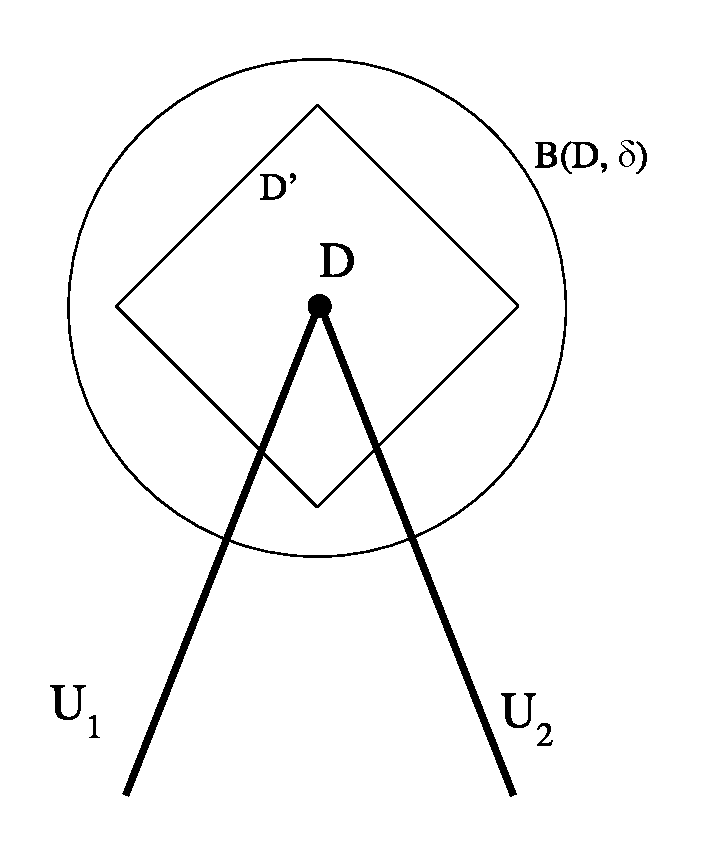
\includegraphics[width=0.24\textwidth]{figs/separated-proof-2} \hfill
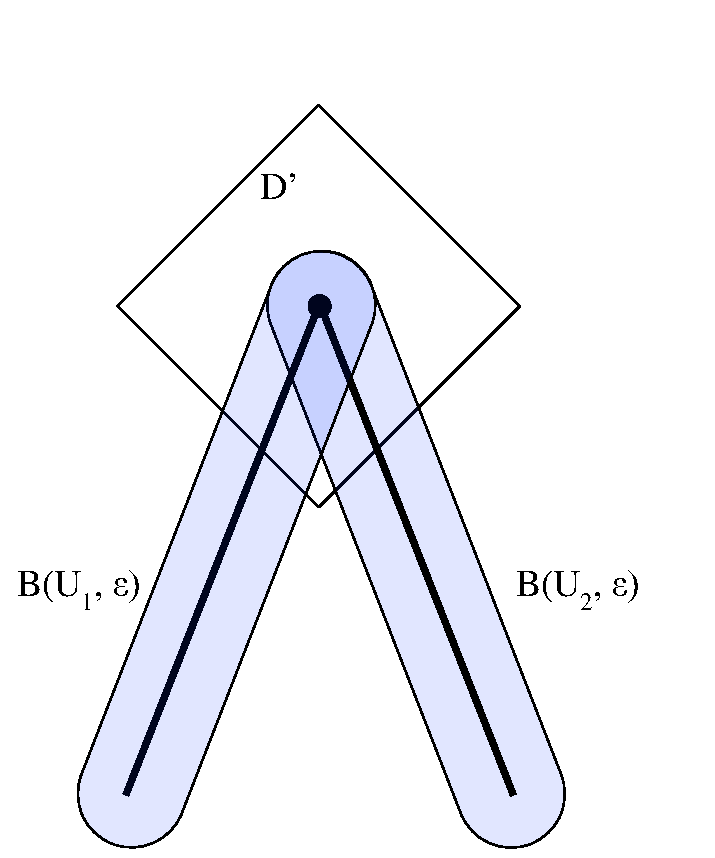
\includegraphics[width=0.24\textwidth]{figs/separated-proof-3} \hfill
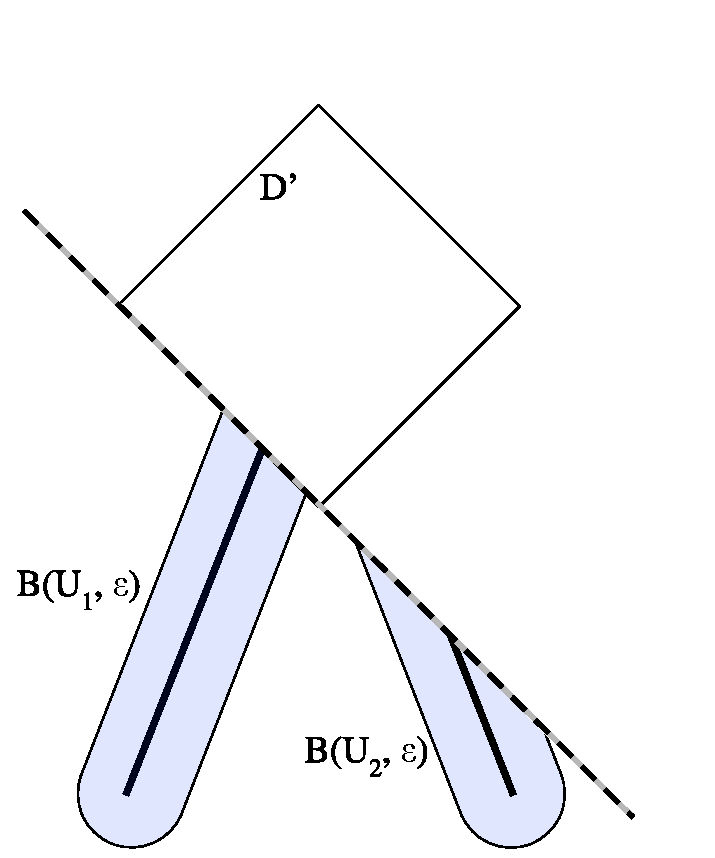
\includegraphics[width=0.24\textwidth]{figs/separated-proof-4} \hfill
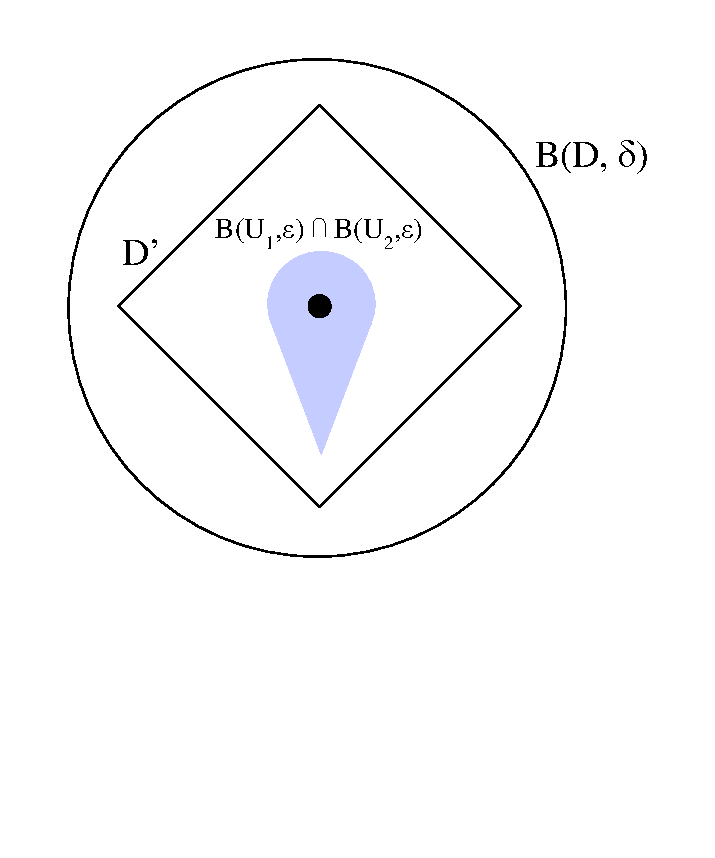
\includegraphics[width=0.24\textwidth]{figs/separated-proof-5}
\end{figure}

\begin{lemma} \label{lemma:thick-empty}
  Let $\{U_j : j \in \mathcal{J}\}$ be a finite collection of nonempty closed, convex sets with $\cap_{j\in\mathcal{J}} U_j = \emptyset$.
  Then for all $\delta > 0$, there exists  $\epsilon > 0$ such that $\cap_{j\in\mathcal{J}} B(U_j,\epsilon) = \emptyset$.
\end{lemma}
\begin{proof}
  By induction on the size of the family.
  Note that the family must have size at least two.
  Let $U_j$ be any set in the family and let $U' = \cap_{j' \neq j} U_{j'}$.
  There are two possibilities.

  The first possibility, which includes the base case where the size of the family is two, is the case $U'$ is nonempty.
  Because $U_j$ and $U'$ are non-intersecting closed convex sets, they are separated by some distance $\epsilon$.
  By Lemma \ref{lemma:thick-nonempty}, for any $\epsilon > 0$, there exists $\delta > 0$ such that $\cap_{j'\neq j} B(U_{j'},\delta) \subseteq B(U', \epsilon/3)$.
  Then we have $B(U_j, \epsilon/3) \cap B(U', \epsilon/3) = \emptyset$.

  The second possibility is that $U'$ is empty.
  This implies we are not in the base case, as the family must have three or more sets.
  By inductive assumption, for small enough $\delta$ we have $\cap_{j' \neq j} B(U_{j'},\delta) = \emptyset$, which proves this case.
\end{proof}


\begin{corollary} \label{cor:thick-intersect}
  There exists a small enough $\epsilon > 0$ such that, for any subset $\{U_j : j \in \mathcal{J}\}$ of $\U$, if $\cap_j U_j = \emptyset$, then $\cap_j B(U_j,\epsilon) = \emptyset$.
\end{corollary}
\begin{proof}
  For each subset, Lemma \ref{lemma:thick-empty} gives an $\epsilon$.
  We take the minimum over these finitely many choices.
\end{proof}

\begin{theorem} \label{thm:small-eps-thick}
  For all small enough $\epsilon$, the epsilon-thickened link $\psi$ (Definition \ref{def:eps-thick-link}) is a well-defined link function from $\R'$ to $\R$, i.e. $\psi(u) \neq \bot$ for all $u$.
\end{theorem}
\begin{proof}
  Fix a small enough $\epsilon$ as promised by Corollary \ref{cor:thick-intersect}.
  Consider any $u \in \R'$.
  If $u$ is not in $B(U,\epsilon)$ for any $U \in \U$, then we have $\Psi(u) = \R$, so it is nonempty.
  Otherwise, let $\{U_j : j \in \mathcal{J}\}$ be the family whose thickenings intersect at $u$.
  By Corollary \ref{cor:thick-intersect}, because of our choice of $\epsilon$, the family themselves has nonempty intersection.
  By Lemma \ref{lemma:calibrated-pos}, their corresponding report sets $\{R_j : j \in \mathcal{J}\}$ also intersect at some $r$, so $\Psi(u)$ is nonempty.
\end{proof}

In the rest of the section, for shorthand, we write $L(u;p) := \langle p, L(u) \rangle$ and similarly $\ell(r;p)$.

\begin{lemma} \label{lemma:exposed-shortest}
  Let $U$ be a convex, closed set and $u \not\in U$.
  Then $\inf_{u^* \in U} \|u-u^*\|$ is achieved by some unique $u^* \in U$.
  Furthermore, $u^*$ is the unique member of $U$ such that $u = u^* + \alpha v$ for some $\alpha > 0$ and unit vector $v$ that exposes $u^*$.
\end{lemma}
\begin{proof}
  Unique achievement of the infimum is well-known.
  (Achievement follows e.g. because the set $U \cap \{u' : \|u - u'\| \leq d(U,u) + 1\}$ is closed and compact, so the continuous function $u' \mapsto \|u-u'\|$ achieves its infimum.
  Uniqueness follows because for two different points $u',u''$ at the same distance from $u$, the point $0.5u' + 0.5u''$ is strictly closer and also lies in the convex set $U$.)
  Now suppose $u = u' + \alpha' v'$ where $v'$ is a unit vector exposing $u'$.
  Then $U$ is contained in the halfspace $\{u'': \langle u'', v'' \rangle \leq \langle u',v' \rangle \}$.
  But every point in this halfspace is distance at least $\alpha'$ from $u$, as $\|u-u''\| \geq \langle v, u - u'' \rangle \geq \langle v, u-u'\rangle = \alpha'$.
  So $u'$ uniquely achieves this minimum distance.
\end{proof}

\begin{lemma} \label{lemma:distance-loss}
  \raft{What I changed: linear ftn $\to$ affine; name the cell $U_f$ for $f$; also name set of functions $\F$, normals $V_f$, etc}
  If $L$ is a polyhedral loss, then for each $p$, there exists a constant $c$ such that, for all $u$,
    \[ L(u;p) - \inf_{u^* \in \R'} L(u^*;p) \geq c \cdot d(\Gamma(p),u) . \]
\end{lemma}
\begin{proof}
  Fix $p$ and let $U = \Gamma(p)$.
  If $u \in U$, then both sides are zero.
  So it remains to find a $c$ such that the inequality holds for all $u \not\in U$.

  $L(\cdot;p)$ is a convex polyhedral function, so it is the pointwise maximum over finitely many affine functions.
  Recall that $\risk{L}(p) = \min_{u} L(u;p)$, the Bayes risk.
  Construct the convex polyhedral function $\hat{L}(\cdot;p)$ by dropping from the maximum those affine functions that are never equal to $L$ for any $u^* \in U$.
  We have $\hat{L}(u^*;p) = \risk{L}(p)$ for all $u^* \in U$ and $\hat{L}(u;p) \leq L(u;p)$ for all $u \not\in U$.
  Now $\hat{L}$ is also a maximum over finitely many affine functions $\F$.
  Each such function $f\in\F$ is equal to $\hat{L}$ above a closed, convex cell $U_f\subseteq\reals^d$ in the power diagram formed by projecting $\hat{L}(\cdot;p)$.
  If $f$ has nonzero gradient, then $U_f \cap U$ is a face of $U$.
  We will prove that there exists $c_f > 0$ such that, for all $u\in U_f$,
    \[ \hat{L}(u;p) \geq \risk{L}(p) + c_f \cdot d(U,u) . \]
  Taking $c$ to be the minimum of $c_f$ over the finitely many $f\in\F$ with nonzero gradient (which covers all points $u \not\in U$) will complete the proof.

  Consider the set of unit vectors $V = \{v \in \reals^d : \|v\|=1\}$ and the boundary of $U$, denoted $\partial U$.
  For any $u^*\in\partial U$, $v\in V$ such that $v$ exposes $u^*$, let
  \raft{NOTE: we need to define ``exposes'' or just phrase in terms of normals: $v$ is normal to $U$ at $u^*$}
  $G_{u^*,v} = \left\{ u^* + \beta v : \beta \geq 0 \right\}$
  be the ray leaving $U$ from $u^*$ in direction $v$.
  % Note that $\{ u : u \not\in U\} \subseteq \cup_{u^*,v} G_{u^*,v}$.
  For each $f\in\F$, we define the set $R_f \subseteq \partial U \times V$ to be the points $(u^*,v)$ such that there exists $\epsilon>0$ with $G_{u^*,v} \cap U_f = G_{u^*,v} \cap B(u^*,\epsilon)$; that is, such that the ray $G_{u^*,v}$ starts its journey in $U_f$.
  Futhermore, define $U^*_{f,v} = \{u^* \in \partial U : (u^*,v)\in R_f\}$ and $V_f = \{v\in V: \exists u^*\in U_f\cap U,\: (u^*,v) \in R_f\}$.
  (That is, $U^*_{f,v}$ is the set of points from which the ray in direction $v$ begins in $U_f$, and $V_f$ is the set of all normal directions in which some ray begins in $U_f$.)
  Finally, define $G_f = \cup_{(u^*,v)\in R_f} G_{u^*,v}$ as the union of all such rays beginning in $U_f$.
  Note that $\cup_{f\in\F} G_f \supseteq \reals^d \setminus U$; this follows as every point not in $U$ is on a normal ray out of $U$, which must begin in some cell $U_f$.

  We will prove the following steps:
  \begin{enumerate}
  % \item For all $u^*\in\partial U$, $v\in V$ such that $v$ exposes $u^*$, there is some $f\in\F$ such that $u^* \in U_f$ and $G_{u^*,v} \cap U_f \neq \{u^*\}$.
  %   (That is, the ray $G_{u^*,v}$ begins its journey away from $U$ within $U_f$.)
    \item For all $f\in\F$, $v\in V_f$, there exists a constant $c_{f,v} > 0$ such that $L(u;p) \geq \risk{L}(p) + c_{f,v} \cdot d(U,u)$ for all $u \in G_{u^*,v}$ and all $u^*\in U^*_{f,v}$.
    \item For all $f\in \F$, the set $V_f$ is compact, and the map $v \mapsto c_{f,v}$ is continuous on $V_f$.
    \item Hence, there is an infimum $c_f > 0$ such that $f(u) \geq \risk{L}(p) + c_f \cdot d(U,u)$ for all $u\in G_f$.
    \item Let $c = \min \{c_f : f\in\F, \nabla f \neq 0\}$; then $L(u;p) \geq \risk{L}(p) + c \cdot d(U,u)$ for all $u \not\in U$.
  \end{enumerate}

  % (1) Follows because $G_{u^*,v}$ is contained in a cell of the power diagram, which is a set of points where $\hat{L}(\cdot;p) = f(\cdot)$. \bo{Should have more justification.}

  (1) Let $\nabla f$ denote the gradient of the affine function $f$.
  Note that because $u^*$ is on the boundary of $U$, we have $f(u^*) = \hat{L}(u^*;p) = \risk{L}(p)$.
  So we can write, using Lemma \ref{lemma:exposed-shortest},
  \begin{align*}
    f(u) &= f(u^*) + (\nabla f)\cdot (u - u^*)  \\
    f(u) &= f(u^*) + (\nabla f)\cdot (d(u^*,u) v)  \\
         &= \risk{L}(p) + c_{f,v} \cdot d(U,u)  \\
  \end{align*}
  where $c_{f,v} = (\nabla f)\cdot v$.
  We must have $c_{f,v} > 0$ because the set $U$ minimizes $L(\cdot;p)$, so $f(u) > f(u^*) = \risk{L}(p)$.
  The result now follows as $L(u;p) \geq \hat L(u;p) \geq f(u)$.

  (2) The intersection $U_f \cap U$ is a face of $U$, and thus decomposes as the union of relative interiors of subfaces, $U_f \cap U = \cup_i \mathrm{ri}(F_i)$.
  For each $i$, let $V_i = \{v\in V: \exists u^*\in \mathrm{ri}(F_i),\: (u^*,v)\in R_f\}$.
  % set $N_U(u^*)$ is the same for all $u^*\in\mathrm{ri}(F_i)$~\cite{lu2008normal}.
  % \raft{That is a total punt reference---not sure the result is in there, but it easily could be!}
  For any $v\in V_i$, we may consider the power diagram restricted to $A$, the affine hull of $\{u + \alpha v: u\in U, \alpha\in\reals\}$.
  As there is some $u^*\in U$ such that $(u^*,v)\in R_f$, in particular, $U_f\cap A$ intersects $A\cap\mathrm{ri}(F_i)$ and thus must contain $A\cap\mathrm{ri}(F_i)$.
  We conclude that $(u',v)\in R_f$ for all other $u'\in \mathrm{ri}(F_i)$.
  \raft{The idea here is that if you can start in $\mathrm{ri}(F_i)$ and move in direction $v$ and land immediately in $U_f$, then you can do that anywhere from $\mathrm{ri}(F_i)$; otherwise $U_f$ intersects only part of $\mathrm{ri}(F_i)$ (at least when restricting to $A$), a contradiction.}
  Thus, we have $\{(u^*,v) \in R_f : u^*\in F_i\} = F_i \times V_i$.
  For closure, pick any $u^*\in \mathrm{ri}(F_i)$, and consider a sequence $\{v_j\}_j$ with $(u^*,v_j)\in R_f$, and corresponding witnesses $\{\epsilon_j\}_j$.
  Then we have $u^* + \epsilon_j v_j \in U_f$ for all $j$, and as $u^*\in U_f$ and $U_f$ is closed and convex, the limiting point must be contained in $U_f$ as well.
  \raft{Thus is totally bogus actually, since the limiting point could be $u^*$ itself.  Need a different approach I think.}
  We have now shown $V_f$ to be the union of finitely many closed convex sets, and thus closed.
  Boundedness follows as $V$ is bounded.
  Finally, $c_{f,v}$ is linear in $v$, and thus continuous.

  Steps (3) and (4) are immediate and complete the proof.
\end{proof}

\begin{theorem} \label{thm:app-eps-thick-sep}
  For small enough $\epsilon$, the $\epsilon$-thickened link $\psi$ (Definition \ref{def:eps-thick-link}) satisfies that, for all $p$, there exists $\delta > 0$ such that, for all $u \in \R'$,
    \[ L(u;p) - \inf_{u^* \in \R'} L(u^*;p) \geq \delta \left[ \ell(\psi(u);p) - \min_{r^* \in \R} \ell(r^*;p) \right] . \]
\end{theorem}
\begin{proof}
  We take the $\epsilon$ thickened link, which is well-defined by Theorem \ref{thm:small-eps-thick}.
  Fix $p$ and let $U = \Gamma(p)$.
  The left-hand side is nonnegative, so it suffices to prove the result for all $u$ such that the right side is strictly positive, i.e. for all $u$ such that $\psi(u) \not\in \gamma(p)$.
  By definition of the $\epsilon$-thickened link, we must have $d(U,u) \geq \epsilon$.
  By Lemma \ref{lemma:distance-loss}, we have $L(u;p) - \inf_{u^*} L(u^*;p) \geq C$ where $C = c\epsilon$ for some $c > 0$.
  This holds for all $u$.
  Meanwhile,
    \[ \ell(\psi(u);p) - \min_{r^*} \ell(r^*;p) \leq \max_{r \in \R} \ell(r;p) - \min_{r^* \in \R} \ell(r^*;p) =: D, \]
  for some constant $D$.
  This also holds for all $u$.
  Set $\delta = \frac{C}{D}$ to complete the proof.
\end{proof}

\begin{proof}[Proof of Theorem \ref{thm:eps-thick-calibrated}]
  The two claims are Theorems \ref{thm:small-eps-thick} and \ref{thm:app-eps-thick-sep}.
\end{proof}


\section{Top-$k$ surrogate}

Consider the surrogate and discrete loss $L^k(u)_y~=~\left(\frac{1}{k} \sum_{i=1}^k (u + \ones - e_y)_{[i]} - u_y \right)_+$ given in Equation~\ref{eq:L-2-surrogate}.

\begin{lemma}\label{lem:top-k-polyhedral}
$L^k$ is a polyhedral loss.
\end{lemma}
\begin{proof}
Observe $L^k$ can be written as the pointwise max of $\binom{n}{k} +1$ terms, where the $\binom{n}{k}$ terms are selecting the $k$ elements of $u + \ones - e_y$, and the max comes from selecting the $u_i$ elements with highest weight.
\end{proof}
%By Lemma~\ref{lem:poly-loss-poly-risk}, we then know that $\risk{L'}$ is also polyhedral.

%We next show that $\U = \{u \in \{0,1\}^n : \|u\|_0 \leq k\}$ is always represented among the optimizers of $L'$. \begin{lemma}\label{lem:top-k-optimal-corners}
%  For all $p \in \simplex$ we have $\prop{L'}(p) \cap \U \neq \emptyset$.
%\end{lemma}
%\begin{proof}
%  Let us first simplify $L'$:
%  \[
%    L'(u)_y = \left( 1 - u_y + \frac{1}{k} \sum_{i=1}^k (u - e_y)_{[i]} \right)_+~.
%  \]
%  Examining this expression, observe that
%  if $u_i < u_{[k+1]}$, then $(u-e_y)_i < (u-e_y)_{[k]}$, as only one entry changes (and decreases) from one to the other.
%  Hence, if $u_i < u_{[k+1]}$, then the index $i$ will not appear in the summation for any $y$, and thus only influences the loss when $y=i$.
%  Now consider the loss of $u'$ which is the same as $u$ but with $u_i' = u_{[k+1]}$.
%  Then $L'(u')_y \leq L'(u)_y$ when $y=i$ and $L'(u')_y = L'(u)_y$ when $y\neq i$.
%  From this we see that without loss of generality, $u_{[k+1]} = \cdots = u_{[n]}$.
%
%  Next, we show that $L'$ is invariant in the $\ones$ direction:
%  \begin{align*}
%    L'(u + \alpha \ones)_y &= \left( 1 - (u_y + \alpha) + \frac{1}{k} \sum_{i=1}^k ((u + \alpha) - e_y)_{[i]} \right)_+\\
%    &= \left( 1 - (u_y + \alpha) + \frac{1}{k}\left[ \alpha k + \sum_{i=1}^k (u - e_y)_{[i]} \right] \right)_+\\
%    &= \left( 1 -u_y + \frac{1}{k}\left[ \sum_{i=1}^k (u - e_y)_{[i]} \right] \right)_+\\
%  &= L'(u)_y~.
%  \end{align*}
%  Thus, without loss of generality, we now have $u_{[k+1]} = \cdots = u_{[n]} = 0$.
%
%  Let $u_{[1..j]} := \sum_{i=1}^j u_{[i]}$.
%  We now claim that for all $y \in \Y$, the minimum of $L(u)_y$ is achieved by some $u \in [0,1]^n$.
%  \raf{Only hole left is the following line.  I think it might not be true.}
%  This follows from the observation that if $u_i > 1$, the the loss only decreases by reporting $u'$ which is equal to $u$ but with $u'_i = 1$.
%  For $u\in[0,1]^n$, the argument to $(\cdot)_+$ is nonnegative, so we can rewrite the expected loss of $L'$ as
%  \begin{align*}
%  	\inprod{p}{L'(u)} &= 1 - \inprod{p}{u} + \frac{1}{k} \left( \sum_{i=1}^k (1 - p_{[i]}) u_{[i]} \right) = 1 + \inprod{\tfrac 1 k \ones - (1+\tfrac 1 k)p}{u}~.
%  \end{align*}
%  As a linear objective over the hypercube, $\inprod{p}{L'}$ must be optimal on some corner of the hypercube, so we conclude $u_{[1]}, u_{[2]}, \ldots, u_{[k]} \in \{0,1\}$.
%  In particular, for all $p \in \simplex$, there is a report $u \in \{0,1\}^n$ optimizing $L'$; since we can take $\|u\|_0 \leq k$ by the above observation that $u_{[k+1]} = u_{[k+2]} = \ldots = u_{[n]} = 0$, some $u \in \U$ must be optimal as well.
%\end{proof}
%
%\raf{Cut this final lemma for now}
% \begin{lemma}\label{lem:top-k-surrogate-embeds}
% $L':\reals^n \to \reals^\Y_+$ embeds $\ell':\R \to \reals^\Y_+$.
% \end{lemma}
% \begin{proof}
%   We can verify $\ell'(r) = L'(\varphi(r))$ for all $r \subseteq [n]$ and $\varphi(r)$ being its conversion from a set to binary vector, so $\varphi(\R) = \{ u \in \{0,1\}^n : \|u\|_1 \leq k \}$.
%   Moreover, by Lemma~\ref{lem:top-k-optimal-corners} and the above equality, respectively, we know that $\inf_{u \in \reals^n} \inprod{p}{L'(u)} = \min_{u \in \varphi(\R)} \inprod{p}{L'(u)} = \min_{r \in \R}\inprod{p}{\ell'(r)}$ for all $p \in \simplex$, and so we conclude that $L'$ embeds $\ell'$.
% \end{proof}


